\chapter{量子谐振子、黑体辐射与光子计数}
\label{ch:oscillator}

\section{谐振子模型与能谱}
前一章用一对给定的能级解释了共振频率。测量分子的振动光谱或用振荡力激发陷阱中的粒子时，
实验还会遇到一个新问题：为什么在低激发区相邻两级的跃迁频率常常近似相同？
经典弹簧的回复力由势能在稳定平衡点的曲率决定。量子理论中，这个曲率决定相邻能级的间距，势能的高阶项则会使能级偏离等间隔。

若一维势能$V(x)$在$x_\eqm$有极小值，令 $\delta x = x - x_\eqm$，
Taylor展开给出
\begin{equation}
    V(x_\eqm + \delta x)
    = V(x_\eqm) + \frac12V''(x_\eqm)(\delta x)^2
        + \frac16V'''(x_\eqm)(\delta x)^3 + \cdots.
\end{equation}
极小点的一阶导数为零，常数项只平移全部能级。
记$m\omega^2 = V''(x_\eqm) > 0$，保留二次项便得到谐振子模型。
截断条件是所占据态上的高阶势能矩阵元相对于相关能级差足够小，
因此“位于平衡点附近”应由态的涨落范围来检验。

分子振动、陷阱中粒子的微小运动和电磁场的单个模式，都能在适当条件下归结为一个二次Hamilton量。
对稳定平衡点附近的一个自由度，舍去常数势能，以 $\op{X}$ 表示相对平衡点的位移算符。保留二次项并取 $\omega > 0$，得到
\begin{equation}
    \op{H} = \frac{\op{P}^2}{2m} + \frac12m\omega^2\op{X}^2.
\end{equation}
较大振幅会探及势阱的非二次部分，相邻能级间距随之可能改变。

$\op{X}$、$\op{P}$分别是位移和正则动量(canonical momentum)；$m$是该正常模式(normal mode)的有效质量(effective mass)，
$\omega$是小振幅角频率。经典弹簧振子的位移为 $x = A\cos(\omega t + \phi)$。
动量 $p = m\dot x$ 比位移相差四分之一个周期，两者合成一个复数便能同时记录振幅和相位：
\begin{subequations}
    \begin{gather}
        x + \frac{\i p}{m\omega} = A\e^{-\i(\omega t+\phi)},\\
        H_{\mathrm{cl}} = \frac{m\omega^2}{2}
            \biggabs{x + \frac{\i p}{m\omega}}^2 .
    \end{gather}
\end{subequations}
相应地，在量子问题中将 $\op{X}$ 与 $\i \op{P}/(m\omega)$ 相加，把能量写成这一组合与其伴随的乘积。
要使乘积以 $\hbar\omega$ 为能量单位，$\op{X} + \i\op{P}/(m\omega)$ 还要乘上 $\sqrt{m\omega/(2\hbar)}$。
记相应的位移、动量尺度为
\begin{subequations}
    \begin{align}
        x_0 &= \sqrt{\frac{\hbar}{2m\omega}},\\
        p_0 &= \sqrt{\frac{m\hbar\omega}{2}},
    \end{align}
\end{subequations}
$x_0, p_0$ 分别具有长度和动量量纲。

\begin{definition}{谐振子的升降算符与数算符}{qm-oscillator-ladder}
    以 $x_0,p_0$ 为单位，定义无量纲的湮灭算符(annihilation operator)
    \begin{equation}
        \op{a} = \frac{1}{2}\Bigp{\frac{\op{X}}{x_0} + \i\frac{\op{P}}{p_0}}.
    \end{equation}
    其伴随算符 $\op{a}\adjoint$ 称为
    产生算符(creation operator)，数算符(number operator) 定义为
    \begin{equation}
        \op{N} = \op{a}\adjoint\op{a}
    \end{equation}
\end{definition}

\begin{corollary}
    易得
    \begin{subequations}
        \begin{align}
            [\op{a},\op{a}\adjoint] &= \one\\
            [\op{N},\op{a}] &= -\op{a}.
        \end{align}
    \end{subequations}
    Hamilton 量可写成
    \begin{equation}
        \op{H} = \hbar\omega\bigp{\op{N} + \one/2}
    \end{equation}
\end{corollary}

\begin{theorem}{一维谐振子的能谱与升降作用}{qm-oscillator}
    取整条实线上只有一个位移自由度的谐振子，其态空间在位置表象中用 $L^2(\RR,\d x)$ 表示。
    它的能量本征态 $\ket n$ 构成一组正交归一基，$n = 0,1,\ldots$，满足
    \begin{subequations}
        \begin{alignat}{2}
            \op{H}\ket{n} &= E_n\ket{n},&\qquad
            E_n &= \hbar\omega\bigp{n + 1/2},\\
            \op{N}\ket{n} &= n\ket{n}.
        \end{alignat}
    \end{subequations}
\end{theorem}

\begin{proof}
    取 $\op{N}\ket{\nu} = \nu\ket{\nu}$ 的归一化本征态，则 $\nu = \mel{\nu}{\op N}{\nu} = \|\op a\ket{\nu}\|^2 \geq 0$。
    由 $\op{N}\op{a} = \op{a}\op{N} - \op{a}$ 有
    $\op{N}(\op{a}\ket{\nu}) = (\nu - 1)\op{a}\ket{\nu}$。
    所得向量若非零，对应的能量比原态低 $\hbar\omega$。
    若基态(ground state)经 $\op a$ 作用后非零，就会得到能量更低的态。于是求基态只需解 $\op a\ket 0 = 0$。
    下一小节将给出它的归一化 Gauss 解。由 $\op N = \op a\adjoint\op a$ 可知该态达到能量下界 $E_0 = \hbar\omega/2$。
    另一方面$[\op{N},\op{a}\adjoint] = \op{a}\adjoint$，升高一次使$\op{N}$的本征值增加1。
    对归一化本征态$\ket{n}$，
    \begin{equation}
        \|\op{a}\adjoint\ket{n}\|^2
        = \mel{n}{\op{a}\op{a}\adjoint}{n}
        = \mel{n}{\op{N} + \one}{n} = n + 1.
    \end{equation}
    从真空逐次升高，并在每一步除以$\sqrt{n + 1}$归一化，得到
    \begin{subequations}
        \begin{align}
            \op{a}\ket{n} &= \sqrt n\ket{n - 1},\\
            \op{a}\adjoint\ket{n} &= \sqrt{n + 1}\ket{n + 1},\\
            \ket{n} &= \frac{(\op{a}\adjoint)^n}{\sqrt{n!}}\ket{0}.
        \end{align}
    \end{subequations}
    不同$n$的态因属于自伴$\op{N}$的不同本征值而正交。
    为验证这些态张成全部态空间，还需排除与每个 $\ket n$ 都正交的非零向量。求得位置波函数后，\ssecref{ss:qm-oscillator-completeness}将完成这一步。
\end{proof}

\section{零点涨落与可测矩阵元}
基态具有零点能 $\hbar\omega/2$，其位置分布有多宽？振荡力又能在什么能级之间激发跃迁？
前一问题取决于基态位移的方差，后一问题取决于位移算符在不同能量本征态之间的矩阵元。两者都可以用升降算符计算。

\subsection{谐振子能量本征态的波函数}
\label{ss:oscillator-position}
若把陷阱中的粒子反复制备在同一能级 $n$，测得的位置分布由 $\psi_n(x) = \braket{x}{n}$ 决定。
在位置表象中，以平衡点为原点，令
$b = \sqrt{\hbar/(m\omega)} = \sqrt 2 x_0$、$\xi = x/b$。
基态满足 $\op a\ket 0 = 0$。取其位置分量，式\eqref{eq:momentum-position}给出动量项中的一阶导数，
\begin{equation}
    \mel{x}{\op a}{0} = \frac{\xi\psi_0(x) + b\psi'_0(x)}{\sqrt 2} = 0.
\end{equation}
换元 $x = b\xi$ 后，$b\psi'_0(x)$ 就是 $\psi_0(b\xi)$ 对 $\xi$ 的导数。积分给出 $\psi_0(x) = C\e^{-\xi^2/2}$。归一化时用 $\d x = b\d\xi$，得到
\[
    1 = \abs{C}^2 b\intR\e^{-\xi^2}\d\xi
    = \abs{C}^2 b\sqrt\pi .
\]
取 $C = 1/(\pi^{1/4}\sqrt b)$ 为正实数。对升高关系 $\op a\adjoint\ket n = \sqrt{n+1}\ket{n+1}$ 也取位置分量，
\begin{equation}
    \label{eq:qm-oscillator-ladder-position}
    \sqrt{n+1}\,\psi_{n+1}(x) = \mel{x}{\op a\adjoint}{n}
        = \frac{\xi\psi_n(x) - b\psi'_n(x)}{\sqrt 2}.
\end{equation}
从基态起连续用两次这个关系，得到
\begin{subequations}
    \begin{align}
        \psi_0(x) &= \frac{\e^{-\xi^2/2}}{\pi^{1/4}\sqrt b},\\
        \psi_1 &= \sqrt2\,\xi\psi_0,\\
        \psi_2 &= \frac{2\xi^2 - 1}{\sqrt2}\psi_0.
    \end{align}
\end{subequations}
乘 $\xi$ 和对 $\xi$ 求导都会改变波函数的奇偶性，所以从偶宇称的基态逐次作用 $\op{a}\adjoint$，所得定态的宇称交替（图\ref{fig:oscillator-states}）。
\begin{figure}[htbp]
    \centering
    \raisebox{-.5\height}{\includegraphics[width=.57\linewidth]{figures/oscillator_states.pdf}}\hfill
    \raisebox{-.5\height}{\tikzfigure{oscillator-ladder}}
    \caption{按相同的 $n$ 对照两图：左图在共同的振幅零线上读节点和符号，右图以虚线所示的势阱底为能量零点，上、下箭头分别表示 $\op{a}\adjoint$、$\op{a}$ 连接的相邻能级。}
    \label{fig:oscillator-states}
    \label{fig:osc-ladder}
\end{figure}

把振幅写成 $\psi_n(x) = C_n H_n(\xi)\e^{-\xi^2/2}$，其中 $H_0 = 1$，$C_0 = 1/(\pi^{1/4}\sqrt b)$。升高一级时，把式\eqref{eq:qm-oscillator-ladder-position}中的常数因子收入 $C_{n+1} = C_n/\sqrt{2(n+1)}$，对多项式和 Gauss 因子的乘积求导便得到
\begin{equation}
    H_{n+1} = 2\xi H_n - H_n'.
\end{equation}
这里的撇表示对 $\xi$ 求导。
由于 $2\xi H_n - H_n' = -\e^{\xi^2}(\e^{-\xi^2}H_n)'$，递推 $n$ 次便得物理学家约定的 Hermite 多项式及归一化波函数
\begin{subequations}
    \begin{align}
        H_n(\xi) &= (-1)^n\e^{\xi^2}\dd[n]{\xi}\e^{-\xi^2},\\
        \psi_n(x) &= \frac{H_n(\xi)\e^{-\xi^2/2}}{\pi^{1/4}\sqrt{2^n n!\,b}} .
    \end{align}
\end{subequations}
分母中的 $\sqrt{n!}$ 来自 $\ket n = (\op a\adjoint)^n\ket 0/\sqrt{n!}$。
利用 $\braket{m}{n} = \delta_{mn}$ 并换元 $\d x = b\d\xi$，得到带权正交关系
\begin{equation}\label{eq:qm-hermite-orthogonality}
    \intR \e^{-\xi^2}H_m(\xi)H_n(\xi)\d\xi
       = \sqrt\pi\,2^n n!\,\delta_{mn}.
\end{equation}

\begin{example}{半谐振子的能谱与定态}{qm-exam-half-oscillator}
    粒子在半轴 $x > 0$ 上的谐振势 $m\omega^2x^2/2$ 中运动，原点处有一面不可穿透的硬墙。求全部能级及相应的归一化波函数，并给出基态能量和相邻能级间隔。

    \par\smallskip\textbf{解}\quad 硬墙要求 $u(0) = 0$。把半轴上的任一本征函数作奇延拓，即令 $u(-x) = -u(x)$。
    延拓后函数和一阶导数在原点连续，且两侧都满足全线谐振子的方程。因此它必是全线的奇宇称本征函数。
    反过来，每个全线奇态限制到右半轴都满足硬墙条件。它在右半轴的概率为 $1/2$，归一化时振幅要乘 $\sqrt 2$。
    用 $j = 0,1,2,\ldots$ 依次编号，取全线量子数 $n = 2j + 1$，便有
    \begin{align*}
        u_j(x) &= \sqrt 2\,\psi_{2j+1}(x), \qquad x > 0,\\
        E_j &= \hbar\omega(2j + 3/2).
    \end{align*}
    基态能量为 $3\hbar\omega/2$，间隔为 $2\hbar\omega$。对任一全线奇态只降一级会得到在原点取非零值的偶态，因而这一步超出了硬墙允许的态。
\end{example}

\subsectionstar{谐振子波函数的完备性与级数截断}
\label{ss:qm-oscillator-completeness}
升降算符生成的能级会不会漏掉某些波包的能量分量？由递推式，$H_n$ 的次数恰为 $n$，所以任意多项式都可用有限个 $H_n$ 线性表示。
若平方可积的 $f(\xi)$ 与每个 $\psi_n$ 都正交，令 $g(\xi) = f(\xi)\e^{-\xi^2/2}$。对每个非负整数 $j$，$g$ 的 $j$ 阶矩都等于零。因此对任意实数 $k$，
\[
    \int_{\RR}\e^{-\i k\xi}g(\xi)\d\xi
       = \sum_{j=0}^{\infty}\frac{(-\i k)^j}{j!}
          \int_{\RR}\xi^j g(\xi)\d\xi = 0 .
\]
这里可以逐项积分，因为绝对值之和以 $\abs{f(\xi)}\e^{-\xi^2/2+\abs{k\xi}}$ 为界，该上界由 Cauchy--Schwarz 不等式可积。
这样 $g$ 的所有 Fourier 分量都为零，反变换给出 $g = 0$，从而 $f = 0$（几乎处处）。这就排除了任何被升降序列遗漏的正交方向。

定态方程还给出逐项求多项式系数的方法。记 $\epsilon = 2E/(\hbar\omega)$，
则 $\psi'' + (\epsilon - \xi^2)\psi = 0$。分离出 Gauss 因子
$\psi = \e^{-\xi^2/2}h(\xi)$可得
\begin{equation}
    h'' - 2\xi h' + (\epsilon - 1)h = 0,
\end{equation}
把 $h$ 展开成幂级数，比较同次幂的系数，得到
\begin{subequations}
    \begin{align}
        h(\xi) &= \sum_{j\geq0}c_j\xi^j,\\
        c_{j+2} &= \frac{2j + 1 - \epsilon}{(j + 2)(j + 1)}c_j.
    \end{align}
\end{subequations}
奇、偶次系数分别递推。势能关于原点对称，可以分别取奇、偶宇称解。
若某一宇称的非零级数一直延续，大阶系数最终同号，且
$(k + 1)c_{2k+s+2}/c_{2k+s} \to 1$，其中 $s = 0$ 或 $1$。
因此在 $\xi > 1$ 时，级数尾项的绝对值从某阶起逐项大于常数乘 $(3\xi^2/4)^k/k!$。
求和后即使乘回 $\e^{-\xi^2/2}$，波函数仍随 $\xi \to \infty$ 增长。平方可积就要求级数截断。
若 $c_n$ 是最后一个非零系数，则 $c_{n+2} = 0$ 给出 $\epsilon = 2n + 1$，
重现 $E_n = \hbar\omega(n + 1/2)$，相应的 $h$ 正比于 $H_n$。

\subsection{位移矩与跃迁}
由$\op{X} = x_0(\op{a} + \op{a}\adjoint)$，$x_0 = \sqrt{\hbar/(2m\omega)}$，直接得到
\begin{subequations}
    \begin{alignat}{1}
        \mel{m}{\op{X}}{n} &= x_0\bigp{\sqrt n\,\delta_{m,n-1} + \sqrt{n + 1}\,\delta_{m,n+1}},\\
        \mel{n}{\op{X}^2}{n} &= x_0^2(2n + 1),\\
        \mel{n}{\op{P}^2}{n} &= \frac{m\hbar\omega}{2}(2n + 1).
    \end{alignat}
\end{subequations}
第一式意味着与 $\op X$ 线性耦合的微弱探针只在相邻谐振子能级间产生一阶跃迁。连续作用两次 $\op X$ 时，两步可以同向升降，也可以一升一降，因此 $\op X^2$ 的非零矩阵元落在主对角线和相隔两格的两条斜带上（图\ref{fig:qm-oscillator-position-matrices}）。
基态的位置与动量均值都为零，二者的标准差满足$\Delta X\Delta P = \hbar/2$。
这些涨落给出有限的平均动能与势能，两项之和就是零点能。

\begin{figure}[htbp]
    \centering
    \tikzfigure{oscillator-position-matrices}
    \caption{谐振子最低十个能级之间的位移矩阵元。横轴 $n$ 为初态，纵轴 $m$ 为末态。左图为 $\op X$，非零元出现在 $m-n = \pm 1$。右图为 $\op X^2$，非零元出现在 $m-n = 0,\pm 2$，主对角线给出各定态的二阶位移矩。两图分别以 $x_0$ 和 $x_0^2$ 为尺度，白格表示零。}
    \label{fig:qm-oscillator-position-matrices}
\end{figure}

\begin{example}{谐振子定态的四阶位移矩}{qm-x-fourth}
    质量为 $m$、角频率为 $\omega$ 的一维谐振子处于定态 $\ket n$。求四阶位移矩 $\mel{n}{\op X^4}{n}$，并给出基态的结果。

    \par\smallskip\textbf{解}\quad 记 $x_0 = \sqrt{\hbar/(2m\omega)}$。由 $\op X = x_0(\op a + \op a\adjoint)$ 连续作用两次，得到
    \begin{equation}
        \op{X}^2\ket{n} = x_0^2\Bigb{
            \sqrt{n(n - 1)}\ket{n - 2}
            + (2n + 1)\ket{n}
            + \sqrt{(n + 1)(n + 2)}\ket{n + 2}}.
    \end{equation}
    对 $n = 0,1$ 略去系数为零的第一项。各分量相互正交，取范数平方，基态给出 $3x_0^4$，一般的 $n$ 给出
    \begin{equation}
        \begin{alignedat}{1}
            \mel{n}{\op{X}^4}{n} &= \|\op{X}^2\ket{n}\|^2\\
            &= x_0^4\bigb{n(n - 1) + (2n + 1)^2 + (n + 1)(n + 2)}\\
            &= 3x_0^4(2n^2 + 2n + 1).
        \end{alignedat}
    \end{equation}
\end{example}

对三个独立、等频自由度，能量是三个振子能量之和，$\op{H} = \hbar\omega(\op{N}_x + \op{N}_y + \op{N}_z + 3\one/2)$。
总量子数$N = n_x + n_y + n_z$的态数是满足该式的有序非负整数三元组数
\begin{equation}
    g_N = \sum_{n_x=0}^{N}(N - n_x + 1) = \frac{(N + 1)(N + 2)}2.
\end{equation}
三个频率不全相等时，同一 $N$ 下的能级一般会分裂。若频率之间存在整数关系，不同的占据数组合仍可能同能。有耦合时，应先求出正常模式。

\section{相干态}
在单个能量本征态中，位置分布始终不变。经典弹簧的质点却会来回振动，振幅和初相位都能测量。
要让位置分布的中心像经典振子一样往返，同时让波包宽度保持在基态的水平，
就需要选择多个能级的振幅和相对相位。下面的一族态恰好有这样的运动，它们各由一个复数标记。

\begin{definition}{相干态}{qm-coherent-state}
    湮灭算符$\op{a}$的归一化右本征态称为相干态(coherent state)：
    \begin{equation}
        \op{a}\ket{\alpha} = \alpha\ket{\alpha},\qquad \alpha \in \CC.
    \end{equation}
    复数$\alpha$同时编码振动幅度和相位。
\end{definition}
把 $\ket{\alpha}$ 在数算符的本征基中展开，系数记为 $c_n$。对比本征方程两边的第 $n$ 个分量得到
$c_{n+1} = \alpha c_n/\sqrt{n + 1}$，从而 $c_n = c_0\alpha^n/\sqrt{n!}$。归一化要求
\[
    1 = \abs{c_0}^2\sum_{n=0}^{\infty}\frac{\abs{\alpha}^{2n}}{n!} = \abs{c_0}^2\e^{\abs{\alpha}^2}.
\]
取 $c_0$ 为正实数，得到
\begin{equation}
    \ket{\alpha} = \e^{-\abs{\alpha}^2/2}\sum_{n=0}^\infty\frac{\alpha^n}{\sqrt{n!}}\ket{n}.
\end{equation}

对数算符 $\op{N}$ 的测量给出整数读数 $n$。由展开系数可求得各读数的概率 $p_n$ 及其均值和方差，
\begin{subequations}
    \begin{alignat}{1}
        p_n &= \e^{-\abs{\alpha}^2}\frac{\abs{\alpha}^{2n}}{n!},\\
        \ave{\op{N}} &= \abs{\alpha}^2,\qquad (\Delta N)^2 = \abs{\alpha}^2.
    \end{alignat}
\end{subequations}
这里 $p_n$ 是均值为 $\abs{\alpha}^2$ 的 Poisson 分布。不同相干态的内积为
\begin{equation}
    \braket{\beta}{\alpha}
    = \exp\Bigp{-\frac{\abs{\alpha}^2 + \abs{\beta}^2}{2} + \beta\conj\alpha}.
\end{equation}
其模为 $\exp(-\abs{\alpha - \beta}^2/2)$，不同相干态有有限的重叠。它们是湮灭算符 $\op{a}$ 的本征态，$\op{a}\adjoint$ 是相应的产生算符。

演化到$t$时刻，
\begin{equation}
    \e^{-\i \op{H}t/\hbar}\ket{\alpha} = \e^{-\i\omega t/2}\ket{\alpha\e^{-\i\omega t}}.
\end{equation}
因此
\begin{subequations}
    \begin{gather}
        \ave{\op{X}} = 2x_0\Re(\alpha\e^{-\i\omega t}),\\
        (\Delta X)^2 = x_0^2,\qquad (\Delta P)^2 = \frac{m\hbar\omega}{2}.
    \end{gather}
\end{subequations}
平均值沿经典振动轨迹运动，方差不随时间变化。
当 $\abs{\alpha} \gg 1$ 时，振幅相对于零点涨落很大；相对涨落随之减小，均值呈现经典振荡。

\section{黑体辐射与Planck分布}
\label{sec:planck}
空腔壁不断吸收和发射辐射。达到热平衡后，腔壁温度决定了从小孔射出的辐射谱。怎样用量子谐振子的能级求出这个频谱？
每个电磁驻波模式相当于一个谐振子。温度决定一个模式的平均热能，把同一频段内所有模式的平均热能相加，就得到这个频段储存的辐射能量。

\subsection{空腔辐射谱与经典能量均分}
\label{ss:blackbody-experiment}

热辐射实验要测量温度固定时，发射功率怎样分配在不同频率区间。
把带有小孔的空腔加热到稳定温度，小孔射出的光经分光元件选频，
再由经过标定的热探测器测量各窄频段的功率。
孔足够小，使辐射逸出不显著破坏腔内热平衡(thermal equilibrium)；
腔壁反复吸收和发射，使频谱主要由温度决定。

1899 年，Lummer 与 Pringsheim 发现，在短波段符合实验的 Wien 辐射公式到了长波段便偏离实测值。
1900 年，Rubens 与 Kurlbaum 选定远红外波长后改变温度，测得在高温下该波段的辐射强度近似正比于绝对温度\cite{history}。
对每个温度，辐射谱都在某一频率达到峰值，在更高频率处逐渐减弱。温度升高时，总辐射功率增大，谱峰移向高频。经典电磁场也有一组腔模式，
但若对每个二次模式采用能量均分，每个模式平均具有$\kB T$的热能。
由于高频模式的数量密度随$\nu^2$增加，
经典能量密度谱也随$\nu^2$增长，对全部频率积分就会发散。

将电磁场量子化后，同一频段内的模式数仍由空腔的大小和形状决定。频率越高，产生一个光子所需的能量 $h\nu$ 越大。当 $h\nu \gg \kB T$ 时，这个模式处于激发态的概率很小，平均热能也随之降低。

\subsection{单模式热分布}
\label{ss:thermal-occupation}

在空腔里固定一个驻波的空间形状和偏振，随时间变化的只剩一个振幅；
Maxwell 方程给这个振幅与弹簧位移同样的简谐振动方程。将这个自由度量子化，
频率 $\nu$ 的模式每增加一级，能量便增加 $\hbar\omega = h\nu$，称为增加一个光子。
电磁场可与壁交换能量。按热平衡的 Boltzmann 权重，
能量为 $E_n$ 的每个微观态具有正比于 $\exp[-E_n/(\kB T)]$ 的概率。
因此相邻占据数的概率比为 $p_{n+1}/p_n = \exp[-h\nu/(\kB T)]$，
零点能在这个比值里抵消。所有占据数的概率相加必须为一，得到
\begin{equation}
    p_n = (1 - \e^{-\beta h\nu})\e^{-n\beta h\nu},\qquad\beta = \frac1{\kB T}.
\end{equation}
$\beta$是逆温度参数，$\kB$为Boltzmann常数。
令$q = \e^{-\beta h\nu}$，有限正温度下$0 < q < 1$。
以真空能为能量零点，配分函数(partition function) $Z$ 为所有权重相加所得的几何级数。
各能级概率为 $p_n = q^n/Z$。把几何级数求和，再对 $q$ 求导，可得
\begin{subequations}
    \begin{align}
        Z &= \sum_{n=0}^\infty q^n = \frac1{1 - q},\\
        \sum_{n=0}^\infty nq^n &= q\dv{Z}q = \frac{q}{(1 - q)^2}.
    \end{align}
\end{subequations}
于是
\begin{equation}
    \bar n = \sum_{n=0}^\infty np_n = \frac1{\e^{\beta h\nu} - 1}.
\end{equation}
热平衡辐射的光子数可变，其化学势(chemical potential)为零。单模式的热能相对真空取值，等于 $h\nu\bar n$。

\subsection{模式计数与辐射量}
\label{ss:radiation-density}

为求大空腔中的模式密度，取边长为 $L$ 的立方盒并施加周期边界条件。波矢(wave vector)的分量满足 $k_i = 2\pi n_i/L$，其中 $n_i$ 为整数，每个格点在三维波矢空间占据体积 $(2\pi/L)^3$。
将半径 $k$、厚度 $\d k$ 的球壳体积 $4\pi k^2\d k$ 除以格点体积，就得到这一层的波矢数。整个球壳已经包含相反的传播方向，每个波矢还有两种横向偏振。计入偏振，再除以盒子体积 $L^3$ 并换成单位频率间隔，得到模式密度
\begin{equation}
    g(\nu) = 2\frac{4\pi k^2}{(2\pi)^3}\frac{\d k}{\nd\nu}
    = \frac{8\pi\nu^2}{c^3},\qquad k = \frac{2\pi\nu}{c}.
\end{equation}
单位体积、单位频率间隔内的能量称为能量密度谱(spectral energy density) $u_\nu$，其值等于模式密度 $g(\nu)$ 乘以单模式的平均热能 $h\nu\bar n$。

各向同性时，每单位立体角分得 $u_\nu/(4\pi)$，乘以光速即得谱辐亮度(spectral radiance) $B_\nu$。两种谱的表达式为
\begin{subequations}
    \begin{align}
        u_\nu &= \frac{8\pi h\nu^3}{c^3}\frac1{\e^{h\nu/(\kB T)} - 1},\\
        B_\nu &= \frac{c}{4\pi}u_\nu.
    \end{align}
\end{subequations}
$B_\nu$的单位是$\unit{\watt\per\metre\squared\per\steradian\per\hertz}$。
它不同于单位面积的出射通量(radiant exitance)；各向同性黑体在向外半球积分给出
\begin{subequations}
    \begin{align}
        M &= \pi\intRplus B_\nu\d\nu
        = \sigma T^4,\\
        \sigma &= \frac{2\pi^5\kB^4}{15h^3c^2}.
    \end{align}
\end{subequations}

上式的几何因子来自辐亮度的定义：
$B_\nu\cos\theta\d\Omega\d\nu$是单位面积向方向$(\theta,\phi)$发出的功率。
因此向外半球的角积分为
\begin{equation}
    \int_0^{2\pi}\d\phi\int_0^{\pi/2}
    \cos\theta\sin\theta\d\theta = \pi.
\end{equation}
在频率积分中换元$x = h\nu/(\kB T)$，
\begin{equation}
    M = \frac{2\pi\kB^4T^4}{h^3c^2}
    \intRplus\frac{x^3}{\e^x - 1}\d x.
\end{equation}
把分母的倒数按公比 $\e^{-x}$ 展成几何级数。各项非负，可以逐项积分；
每项对 $x$ 作三次分部积分，得到
\begin{equation}\label{eq:qm-planck-integral}
    \intRplus\frac{x^3}{\e^x - 1}\d x
    = \sum_{r=1}^\infty\intRplus x^3\e^{-rx}\d x
    = 6\sum_{r=1}^\infty\frac1{r^4}
    = 6\zeta(4) = \frac{\pi^4}{15}.
\end{equation}
最后一步采用 Riemann $\zeta$ 函数的已知值 $\zeta(4) = \pi^4/90$。

低频$h\nu \ll \kB T$恢复每模式$\kB T$的经典结果，高频受指数抑制。

同一小段光谱用频率或波长表示时，所含的辐射功率相同，故 $B_\lambda\,\d\lambda = B_\nu\,\abs{\d\nu}$。代入 $\nu = c/\lambda$ 得
\begin{equation}
    B_\lambda = B_\nu(c/\lambda)\frac{c}{\lambda^2}
    = \frac{2hc^2}{\lambda^5}\frac1{\e^{hc/(\lambda\kB T)} - 1}.
\end{equation}
取 $x = hc/(\lambda\kB T)$，$B_\lambda$ 的极值条件为 $x = 5(1 - \e^{-x})$。代入正根 $x_\lambda = 4.965114\ldots$，得到 Wien 位移定律
\begin{equation}
    \lambda_{\max}T = \frac{hc}{x_\lambda\kB}
       \simeq \qty{2.898e-3}{\metre\kelvin}.
\end{equation}
升温使峰值移向短波（图\ref{fig:planck-wavelength}）。
\begin{figure}[htbp]
    \centering
    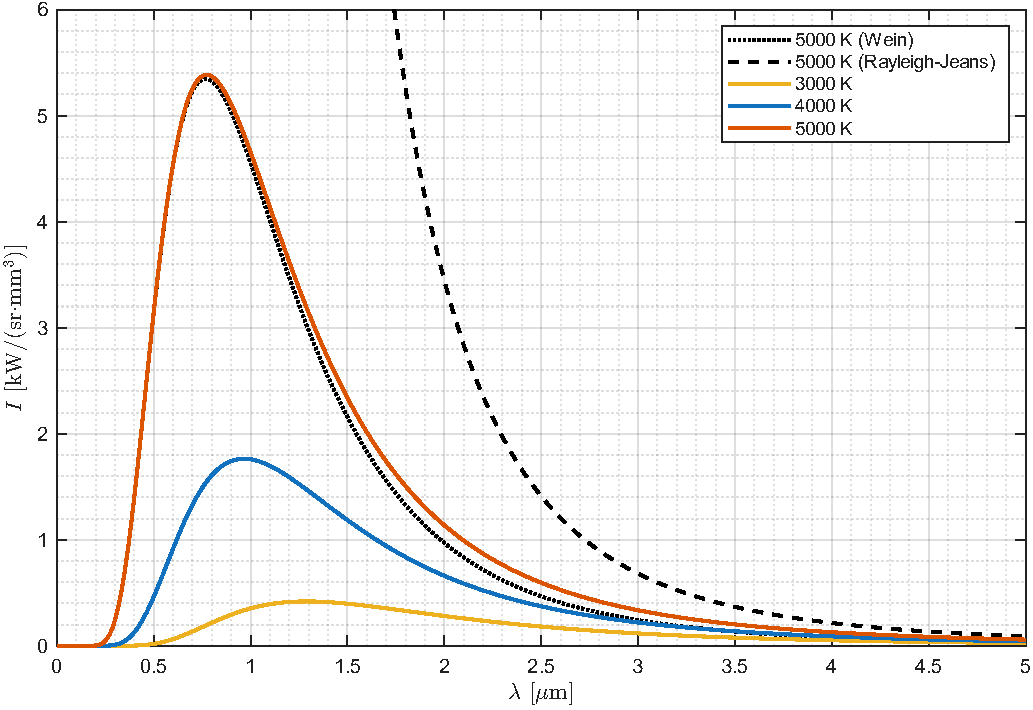
\includegraphics[width=.65\linewidth]{figures/blackbody.pdf}
    \caption{不同温度下的黑体谱辐亮度 $B_\lambda$ 随波长的变化。与最高温度的曲线相比，Wien近似适用于短波一侧，Rayleigh--Jeans近似适用于长波一侧。}
    \label{fig:planck-wavelength}
\end{figure}
若改求 $B_\nu$ 的峰值，无量纲变量 $x = h\nu/(\kB T)$ 满足 $x = 3(1 - \e^{-x})$。从频率谱换成波长谱时，Jacobian也随波长变化，两种谱密度的峰值波长与峰值频率应分别由相应的极值条件确定。
这些公式要求热平衡和黑体吸收发射条件，非平衡激光没有Planck分布。

\section{光子计数与反关联}
\label{sec:photoncount}
热辐射谱给出各频段的平均能量。弱相干光和低重复率的单光子源都能给出稀疏计数，怎样知道光子是否成对到达？
\phantomsection\label{exp:qm-photon-anticorrelation}
1986 年，Grangier、Roger 与 Aspect 利用原子级联跃迁先后发出的两个光子。探测到第一个光子时打开计数窗口，让第二个光子进入分束器。两端的探测器分别记录单计数，若在同一窗口内两端都点击，就记为一次符合(coincidence)\cite{grangier}。

一次触发后，两路各自点击的概率记为 $p_1,p_2$，符合概率记为 $p_{12}$。
在低效率、背景可忽略且时间窗一致时，$p_{12}/(p_1p_2)$ 消去效率和分束比，给出归一化二阶关联。
若该比值小于一，符合少于独立点击的预期，称为反关联(anticorrelation)。实验中反关联最明显的一组数据给出 $p_{12}/(p_1p_2) = 0.18 \pm 0.06$\cite{grangier}。

理想光电探测的单次计数率正比于平均光子数 $\ave{\op{a}\adjoint\op{a}}$。
\begin{definition}{单模式的零延迟二阶关联}{qm-photon-correlation}
    对平均光子数 $\ave{\op{N}} > 0$ 的单个模式，归一化零延迟二阶关联函数(second-order correlation function)为
    \begin{equation}
        g^{(2)}(0) = \frac{\ave{\op{a}\adjoint \op{a}\adjoint \op{a}\op{a}}}{\ave{\op{a}\adjoint \op{a}}^2}
        = \frac{\ave{\op{N}(\op{N} - \one)}}{\ave{\op{N}}^2}.
    \end{equation}
\end{definition}
模式中有 $n$ 个光子时，吸收第一个光子后还剩 $n - 1$ 个。连续吸收两次的计数率正比于 $n(n - 1)$，所以分子取这个乘积的平均值。分母用平均光子数的平方给出两次独立探测的计数基准。

在含有 $n \geq 1$ 个光子的数态 $\ket{n}$ 中，测量 $\op{N}$ 总是得到 $n$，故 $g^{(2)}(0) = 1 - 1/n$。
对 $\alpha \ne 0$ 的相干态，连续两次用 $\op{a}\ket{\alpha} = \alpha\ket{\alpha}$ 得分子 $\abs{\alpha}^4$，与分母相等，故比值为一。
对温度 $T > 0$ 的单模式热态(thermal state)，$g^{(2)}(0) = 2$，因为对几何级数求两次导数有
\begin{equation}
    \ave{\op{N}(\op{N} - \one)}
    = (1 - q)q^2\dv[2]{}q\frac1{1 - q}
    = \frac{2q^2}{(1 - q)^2} = 2\bar n^2.
\end{equation}
$\ket{1}$不能在理想分束后触发两个单光子吸收探测器的同次符合；
经典正随机强度则由$\ave{I^2} \geq \ave{I}^2$给出$g^{(2)}(0) \geq 1$。
实验判别反关联需控制暗计数、多光子成分、时间窗和背景\cite{grangier}。
弱相干光即使平均光子数很小，仍给出 $g^{(2)}(0) = 1$。

\begin{example}[unbreakable]{谐振子热态的平均能量}{qm-oscillator-thermal-energy}
    角频率为 $\omega$ 的谐振子与温度为 $T$ 的热库平衡。分别以势阱底和基态能量为零点，求平均能量及其在 $T\to 0$ 时的极限。两种约定给出的热容有何关系？

    \par\smallskip\textbf{解}\quad 记 $\beta = 1/(\kB T)$。从势阱底计，$E_n = \hbar\omega(n + 1/2)$，
    配分函数和平均能量为
    \begin{subequations}
        \begin{alignat}{1}
            Z &= \sum_{n=0}^{\infty}\e^{-\beta\hbar\omega(n+1/2)}
                = \frac{\e^{-\beta\hbar\omega/2}}
                    {1 - \e^{-\beta\hbar\omega}},\\
            \ave{\op{H}} &= -\pv{\ln Z}{\beta}
                = \frac{\hbar\omega}{2}
                    + \frac{\hbar\omega}{\e^{\beta\hbar\omega} - 1}.
        \end{alignat}
    \end{subequations}
    以真空为能量零点时，$\op{H}' = \op{H} - \hbar\omega\one/2$。各态的 Boltzmann 权重与配分函数都乘以 $\exp(\beta\hbar\omega/2)$，归一化概率因而相同，热容和跃迁概率也相同。
    当 $T \to 0$ 时，平均占据数 $\bar n \to 0$，以阱底为零点的平均能量趋于 $\hbar\omega/2$；以基态为零点的平均能量 $\hbar\omega\bar n$ 趋于零。此时热辐射通量也趋于零。
\end{example}

\reading{Hermite 多项式的权函数与归一化可查\href{https://dlmf.nist.gov/18.3}{NIST 数学函数手册第18.3节}。
    光子的热占据见 Feynman 第 III 卷第 4 章\cite{feynman4}。下一章用升降算符求角动量谱。}
